\section{Ejercicio 5}

$$
F(A,B,C,D) = \prod(1,3,5,7,13,15)
$$

\subsection{Expresión mínima}

\begin{figure}[H]
    \centering
    \begin{karnaugh-map}[4][4][1][$D$][$C$][$B$][$A$]
        \maxterms{1,3,5,7,13,15}
        \implicant{1}{7}
        \implicant{5}{15}
    \end{karnaugh-map}
    \caption{Mapa de Karnaugh para la función}
\end{figure}

\begin{align*}
F(A,B,C,D) &= (A+\overline{D})(\overline{B}+\overline{D})\\
F(A,B,C,D) &= A\overline{B} + \overline{D} 
\end{align*}

\subsection{Simulación en Falstad}
\begin{figure}[H]
    \centering
    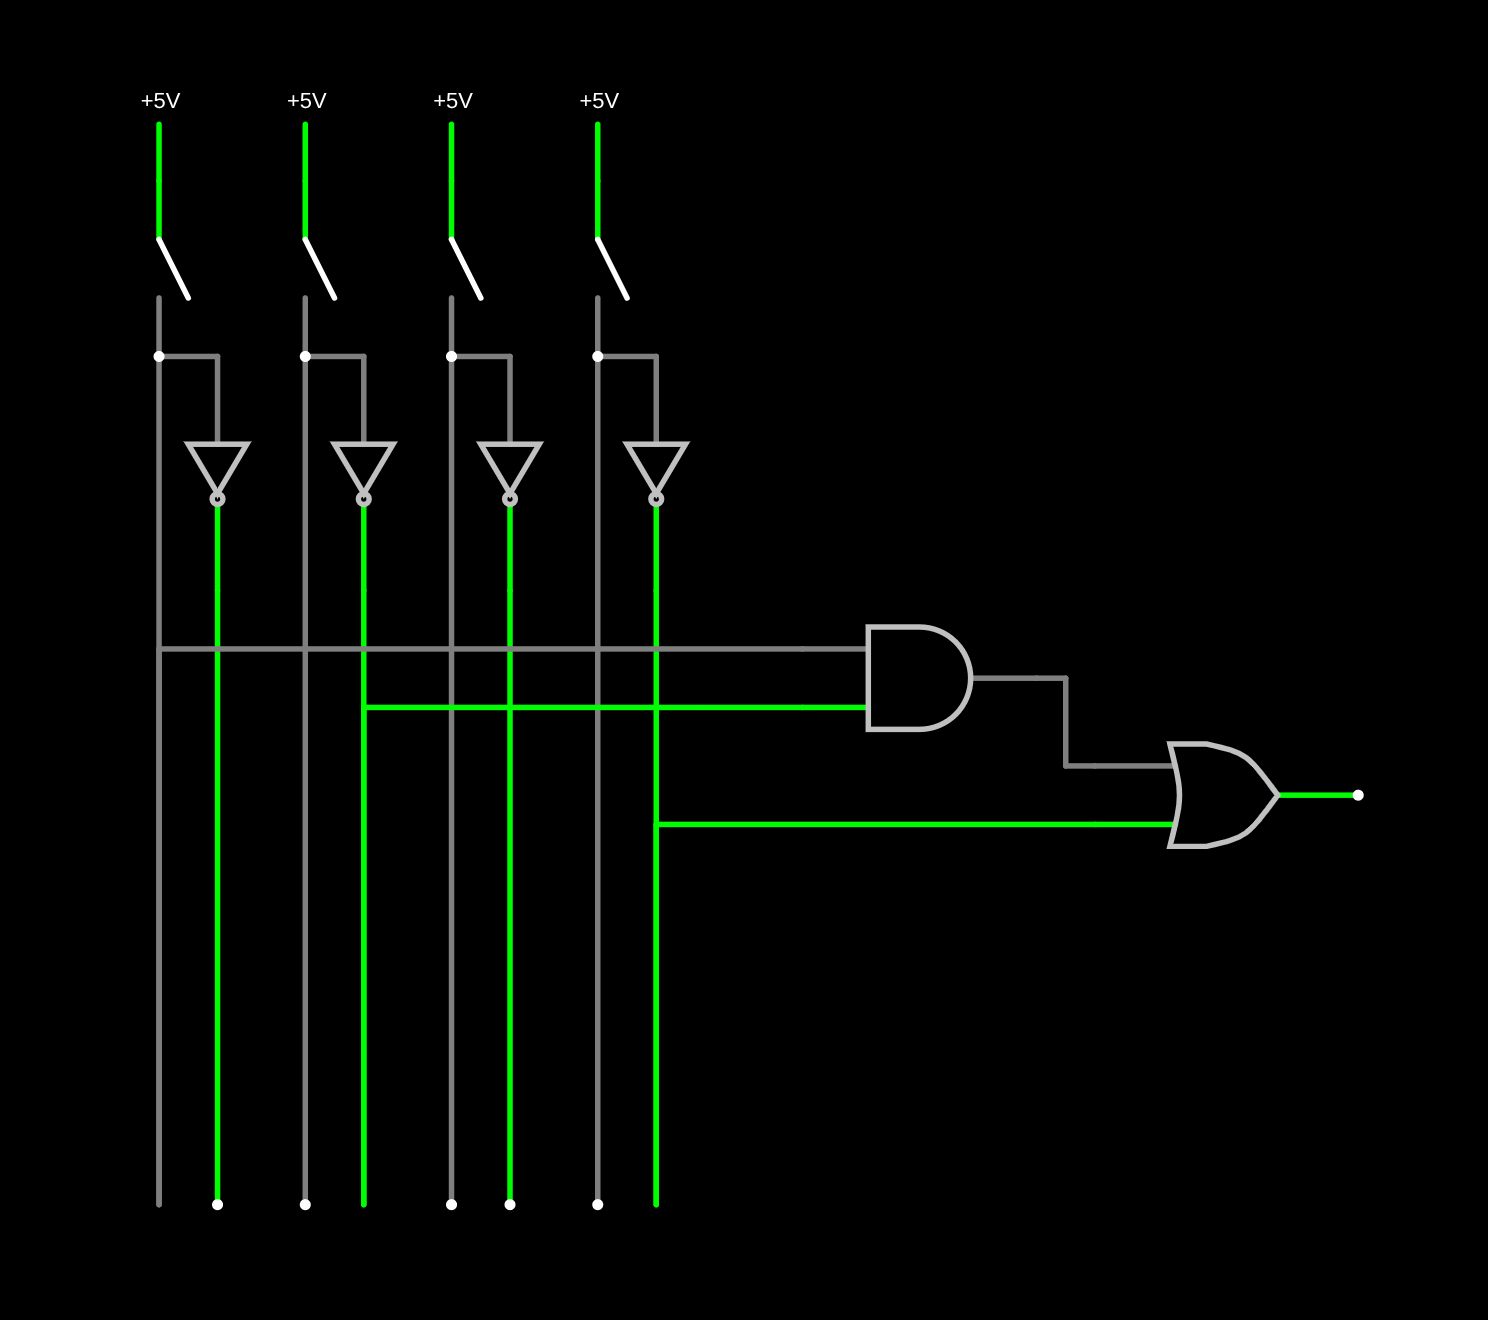
\includegraphics[width=0.6\textwidth]{img/Falstad/ej7.png}
    \caption{Simulación de la función en Falstad}
\end{figure}

\subsection{Descripción en Verilog}

\begin{Verbatim}[ frame=single, fontsize=\small, baselinestretch=1.2 ]
module ej5 (
    input A,
    input B,
    input C,
    input D,
    output F
);

assign F = A & ~B | ~D ;

endmodule
\end{Verbatim}

\subsection{Captura del RTL}
\begin{figure}[H]
    \centering
    
\includegraphics[width=0.8\textwidth]{img/Xilinx/ej7.png}
    \caption{Captura del RTL en Xilinx}
\end{figure}